\chapter{Design}

As intermixing is the method required, two versions of the prototype will be designed.

\section{Initial Designs}
This section will present the initial concept ideas, and explain how they fulfil the design requirements found in the analysis. Finally, the concept for the final design will be chosen.

\subsection{Concepts}

\begin{itemize}
    \item Get-To-Work-Simulator:\\
    In "Get-To-Work-Simulator", the user will try to get to work as efficiently as possible, through a number of options presented throughout the experience. The user will play through mini-games, and decide how to get from A to B. Get-To-Work-Simulator will focus on improving how the individual gets about in their daily lives, and try to get more people to choose bicycle or public transportation, which the analysis explained is a significant cause for pollution.\\
    INSERT GET-TO-WORK-SIMULATOR PICTURE HERE\\
    \item House:\\
    In "House", the users finds themselves in a regular house. As they start their day, they will be presented with a series of tasks for them complete. These tasks are inspired by the mechanics found in the popular VR-game "Job simulator", however they are changed to be relevant to climate change.\\
    INSERT HOUSE PICTURE HERE\\
    \item Local-Community-God-Simulator:\\
    Local-Community-God-Simulator
    \item 60 seconds climate saver:\\
    60 seconds climate saver
    \item Narrative Driver:\\
    Narrative Driver
    \item Making Mars Great Again:\\
    Making Mars Great Again.
\end{itemize}

\subsection{Choosing the concept}
Narrative driver is chosen because nice.

\section{Final design}
Narrative driver explained overall

\subsection{Narration}

\subsection{Graphics}

\subsection{Environment}

\section{Usability test}
    For discerning the usability of the interactions in the design, a simple test using the SUS scale questionnaire, was conducted. The test subject were told to put the Virtual Reality headset on their head, and got one controller handed to their primary hand. The subject were then observed during the test, and afterwards instructed to fill out the SUS questionnaire, and then concluding the test, with any questions answered by the researchers.
\subsection{Test setup}
    The setup for the Usability test (seen in \autoref{fig:usabilitySetup}), using the SUS questionnaire, where the test subject, going through the test, were positioned in front of the monitor with the HMD on their head. The observer sitting on a couch nearby, were noting any miscellaneous usability related things.
\begin{figure}[H]
    \centering
    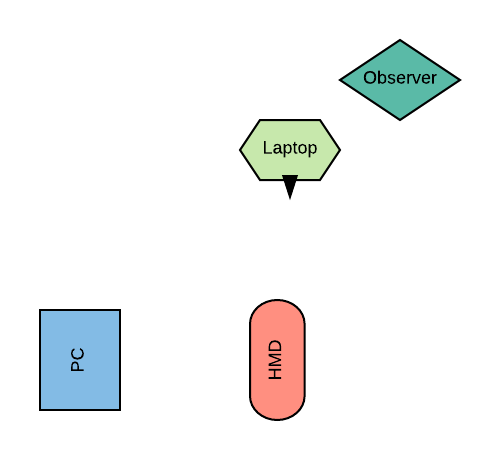
\includegraphics[width=0.6\linewidth]{figure/Design/UsabilitySetup.png}
    \caption{The setup of the usability test, with the \color{red}{HMD/User}, \color{blue}{PC}, \color{teal}{Observer}, and \color{green}{Laptop for SUS}}
    \label{fig:usabilitySetup}
\end{figure}

\subsection{Test results}
    Very usable, much burger eating, nice means.
